\section{Background}
\label{sec:background}

\subsection{Stateful Coding-Agent Execution}

ReAct interleaves model reasoning with actions and observations from an
external environment~\cite{react}. Coding agents such as SWE-agent and
OpenHands repeatedly inspect repositories,
edit files, invoke shell commands, and run tests~\cite{sweagent,openhands}.
Each tool call can consume source edits, generated artifacts, or configuration
changes left by earlier calls. The filesystem therefore carries
progress across the task. At the same time, the agent context---the messages
supplied to subsequent model requests---records calls and their results.
A reported test outcome, for example, describes a particular filesystem
version. After recovery, the observations supplied to the agent should
therefore describe the file state that remains.

Toolformer incorporates API results into subsequent token
generation~\cite{toolformer}. Reflexion retains textual feedback for later
attempts, while MemGPT moves information between memory tiers and the
active model context~\cite{reflexion,memgpt}. Software-engineering systems such as
AutoCodeRover, Agentless, and HyperAgent combine localization, editing, and
validation~\cite{autocoderover,agentless,hyperagent}.
SWE-Bench and Terminal-Bench evaluate agents through executable repository
and command-line tasks~\cite{swebench,tbench}.
SWE-Gym trains agents and verifiers in executable repository
environments~\cite{swegym}. FeatureBench and SWE-EVO extend evaluation to
complex feature development and sustained, multi-file software
evolution~\cite{featurebench,sweevo}. These workflows accumulate both modified
files and observations that later decisions reuse.

An error can affect both forms of state. A later tool call can read an incorrect
file, or the model can reuse an incorrect value from a tool result in a later
request. These effects therefore extend to subsequent calls that
consume the faulty state or reuse affected results. Recovery determines how
much valid work survives by choosing which calls to withdraw from both
histories.

\subsection{Recovery Support for Stateful Agents}

Classical rollback-recovery protocols use checkpoints and logs to resume
consistent execution after failures~\cite{rollbacksurvey}. Process
checkpointing and file transactions provide underlying state-management
mechanisms~\cite{criu,dmtcp,valor,txfs}. We classify agent-facing recovery
interfaces by the scope of their rollback: selected effects, temporal
checkpoint, turn checkpoint, and whole branch.
Figure~\ref{fig:motivation-rollback-example} illustrates these four scopes
on six calls across three turns. Call 4 writes an incorrect value to A,
and Call 6 reads it; the updates to B, C, D, and E remain valid.

\begin{figure}[t]
  \centering
  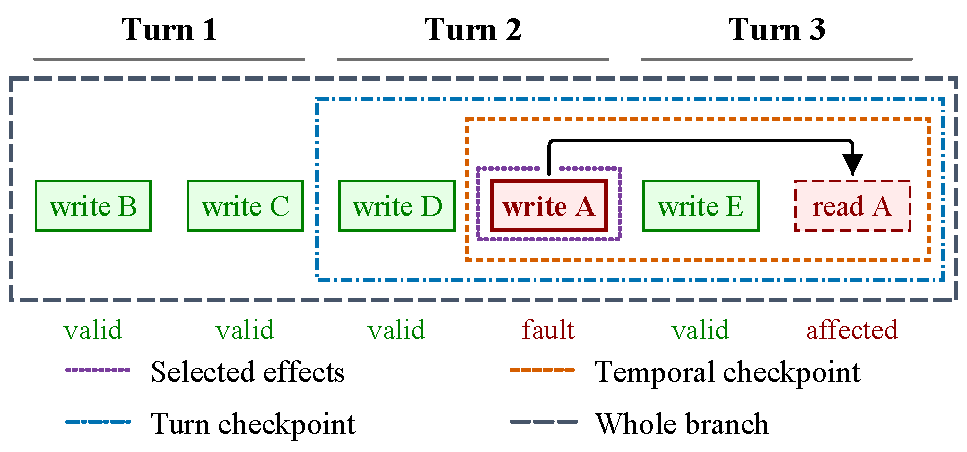
\includegraphics[width=0.8\linewidth]{FIG-Recovery-Granularity.pdf}
  \caption{\textbf{Recovery granularity over interleaved tool calls.}
  \small\emph{Red calls are faulty or affected; green calls are independent.
  Four outline styles mark selected effects, a temporal suffix, a
  turn-boundary suffix, and the whole branch. The arrow denotes dependency.}}
  \label{fig:motivation-rollback-example}
\end{figure}

\textbf{Selected effects.}
Semisolates let callers inspect, selectively apply or discard, filter, and
stack filesystem effects~\cite{try-osdi26}. Their tracing interface also
extracts dependencies. In the example, discarding the faulty write to A
alone leaves the later read affected. Discarding a file effect therefore
also calls for a decision about which dependent agent calls and
observations to withdraw.

\textbf{Temporal checkpoint.}
These interfaces restore a saved environment version. Waypoint captures filesystem and
process state together~\cite{waypoint,waypoint-project}. DeltaBox pairs
DeltaFS layer switching with DeltaCR process restoration to return both
forms of state to the same checkpoint~\cite{deltabox}.
Planarian also coordinates supported remote effects through compensating
operations~\cite{planarian}. In the example, restoring the point before
Call 4 withdraws the last three calls, including the independent update to E.

\textbf{Turn checkpoint.}
These interfaces place recovery points at agent-turn boundaries. Crab uses
observed OS effects to select the state to capture and overlaps capture
with execution~\cite{crab}. AgentRewind restores aligned filesystem and
agent-context checkpoints and retains lessons from abandoned
attempts~\cite{agentrewind}. In the example, restoring the start of Turn 2
also removes the independent update to D.

\textbf{Whole branch.}
These interfaces discard a complete speculative branch or transaction.
BranchFS provides nested copy-on-write branches with commit/abort~\cite{branchfs}.
Cordon stages local mutations and external effects, tracks result lineage,
and validates the composed flow before commit; local rollback restores
pre-transaction state~\cite{cordon}. Whole-branch recovery in the example
withdraws all six calls, including all four independent updates.

Other mechanisms support isolation and dependency-aware execution.
Sandlock confines agent-invoked code with a copy-on-write work
directory~\cite{sandlock}. hS uses dependencies to revoke and re-execute
affected speculative subprocesses while preserving sequential
semantics~\cite{hs-osdi26}. Provenance systems record how outputs derive
from earlier actions~\cite{pass,beep}; RETRO uses an action-history graph
to undo unwanted actions and selectively re-execute affected legitimate
actions~\cite{retro}.

Table~\ref{tab:granularity} compares the scopes on two recovery goals:
removing all affected calls and preserving all independent work. A turn
checkpoint policy can preserve unaffected turns, but loses independent
calls inside withdrawn turns. A temporal checkpoint policy can also
discard independent work in later unaffected turns. State coverage is
separate from rollback scope:
Waypoint, for example, restores files and processes, whereas AgentRewind
restores files and agent context.

\begin{table}[!htbp]
\centering
\footnotesize
\setlength{\tabcolsep}{2pt}
\renewcommand{\arraystretch}{1.2}
\begin{tabular}{@{}lccc@{}}
\toprule
 & & \multicolumn{2}{c}{\textbf{Keep independent work}} \\
\cmidrule(l){3-4}
\textbf{Recovery scope} &
\shortstack{\textbf{Remove all}\\\textbf{affected calls}} &
\shortstack{In unaffected\\turns} &
\shortstack{In affected\\turns} \\
\midrule
Selected effects (\trycmd) & $\times$ & $\checkmark$ & $\checkmark$ \\
Temporal checkpoint (DeltaBox) & $\checkmark$ & $\times$ & $\times$ \\
Turn checkpoint (Crab) & $\checkmark$ & $\checkmark$ & $\times$ \\
Whole branch (BranchFS) & $\checkmark$ & $\times$ & $\times$ \\
\bottomrule
\end{tabular}
\par\vspace{1pt}
\begin{minipage}{\linewidth}
\footnotesize\raggedright
$\checkmark$: guaranteed by the scope with exact affected-call information;
$\times$: no general guarantee. Retention means keeping \emph{all}
independent work, including work after the fault. With selected effects,
recovery removes the faulty file effect alone, without expanding to dependent calls.
\end{minipage}
\caption{\textbf{Recovery completeness and independent-work retention.}
The scopes differ in whether they remove dependent calls and how much
independent work they can preserve.}
\label{tab:granularity}
\end{table}

\begingroup\clubpenalty=10000
These scopes can discard independent calls. We next measure that loss
and examine how dependencies enable selective rollback.
\par\endgroup
